%-----------------------------------
%
\chapter{Assembly}
%
%-----------------------------------

\AY{Different ways to put the above layers together/ordering them. Simulating RASPS and etc can go here?}


\section{Induction Heads}

\LS{Will write}

\section{n-grams}

\AY{Will write}

\section{Computing MOD without positional encodings}

\WM{Will write}

\section{Dyck Language}
\AX{Will write}\CW{Will also write}
The language \dyckk{k} comprises all strings of well-nested brackets, where at most $k$ distinct kinds of bracket may occur. The following context-free grammar generates \dyckk{k}:\begin{align*}
    S \rightarrow & (_i S)_iS \; \text{for}\, i \in [k]\\
    S \rightarrow & \epsilon
\end{align*}
While \dyckk{k} has been shown to be hard for transformers under certain assumptions~\citep{hahn-2020-theoretical,bhattamishra2020ability}, it is possible to construct a \SMAT{} transformer to recognize \dyckk{1}~\citet{bhattamishra2020ability}. Moreover, \dyckkd{k}{D}, the Dyck language with \textit{nesting depth} bounded by $D$, can be recognized by a $(D{+}1)$-layer \UHAT Transformer and can be generated by a $2$-layer \SMAT{} transformer~\citep{yao2021self}.\footnote{\citet{yao2021self} note that either construction can be adapted for the other purpose.}
\subsection{SMAT for Dyck-1}

\subsection{UHAT transformer for Dyck-k-D}
\CW{Will write}
The following construction appears in section 5.1 of~\citet{yao2021self}.
The main idea is that membership in \dyckk{k} can be checked by recursively removing matched pairs of brackets, starting at the most deeply nested brackets and moving outward. The string is in \dyckk{k} iff all brackets can be matched without encountering an out-of-place bracket. Each step of this process can be implemented by a transformer layer in which each token only attends to the nearest bracket that has not been matched (removed) at an earlier step. Since we are considering \dyckkd{k}{D}, we have an \textit{a priori} bound of $D$ on the maximum nesting depth, so we can implement this procedure with a $D + 1$ layer transformer. 

To implement this procedure,~\citet{yao2021self} use the intermediate representations to maintain and update the \textit{state} for each token position. A bracket's state can be one of \textit{Unmatched} (when the bracket's match has not yet been found), \textit{Matched} (when the bracket's match has been found), or \textit{Error} (when the bracket match has not been found within $D$ sets of nesting bracket, which implies the string is not in \dyckkd{k}{D}). In addition to this mutable state, the intermediate representations contain bookkeeping information that is passed unchanged between layers using residual connections. Formally, the intermediate representation at position $i$ after layer $\ell$ is denoted $\mathbf{x}_{i,\ell} = [\mathbf{t}_i, o_i, p_i, m_{i,\ell}, e_{i,\ell}]$ and comprises:\begin{itemize}
    \item $\mathbf{t}_i \in \mathbb{R}^{\lceil\log k\rceil}$: The \textit{bracket type embedding}, which encodes which of the $k$ kinds of brackets appears at input position $i$ (or if the token is one of the special BOS or EOS tokens).
    \item $o \in \{0,1\}$: The \textit{openness} bit, which is $0$ for open brackets (or BOS) and $1$ otherwise.
    \item $p_i \in \mathbb{R}$: The \textit{positional encoding} $p_i = i/n$.
    \item $m_{i,\ell} \in {0,1}$: The \textit{match} bit which starts as $0$ (unmatched) and is updated to $1$ (matched) when the token's match is found.
    \item $e_{i,\ell} \in {0,1}$: The \textit{error} bit which starts as $0$ and is updated to $1$ if an out-of-place bracket is found.
\end{itemize}
Each intermediate representation has dimensionality $d_{model}$. The construction consists of $D$ identical self-attention and FFN blocks that update the state at each token position, followed by one additional self-attention and FFN block that outputs success or failure depending on the state at each token.

\subsubsection{First D layers}
The first $D$ layers are identical and use three attention heads:\CW{add reference to multihead attention}\begin{itemize}
    \item $\mathrm{Att}^{\mathrm{id}}$: Passes the representation from the previous layer through unchanged.
    \item $\mathrm{Att}^{\mathrm{left}}$: Attends to the the nearest unmatched token to the left of the current position.
    \item $\mathrm{Att}^{\mathrm{right}}$: Attends to the the nearest unmatched token to the right of the current position.
\end{itemize}

We will now describe the the $\ell^{\mathit{th}}$ layer (where $\ell \in [D]$). 
To reduce notational clutter, we will denote $\mathbf{x}_{i}=\mathbf{x}_{i,\ell-1}$ ($i^\mathit{th}$ input vector to layer $\ell$), $m_i = m_{i,\ell-1}$ ($i^\mathit{th}$ position's match bit produced at previous layer), $\mathbf{a}_i=\mathbf{a}_{i,\ell}$ ($i^\mathit{th}$ attention output at layer $\ell$), and $\mathbf{y}_{i} = \mathbf{x}_{i,j}$ (the output of layer $\ell$). The attention output at the $i^{\mathit{it}}$ position is the concatenation of each head's attention output, which we write as $\mathbf{a}_{i} = [\mathbf{a}_{i}^{\mathrm{id}}, \mathbf{a}_{i}^{\mathrm{left}}, \mathbf{a}_{i}^{\mathrm{right}}]$.

The identity attention head $\mathrm{Att}^{\mathrm{id}}$ is defined such that $\mathbf{a}_{i}^{\mathrm{id}} = \mathbf{x}_i$. \CW{Insert ref to identity attention section of cookbook.}

To attend to the nearest unmatched token to the left, $\mathrm{Att}^{\mathrm{left}}$ uses future-positional masking and defines query, key, and value matrices $Q \in \mathbb{R}^{1 \times d_{model}}$, $K \in \mathbb{R}^{1 \times d_{model}}$, and $V \in \mathbb{R}^{d_{model} \times d_{model}}$ such that:\begin{align*}
    Q\mathbf{x}_{i} & = 1 \in \mathbb{R}\\
    K\mathbf{x}_{i} & = p_i - m_i \in \mathbb{R}\\
    Q\mathbf{x}_i & = \mathbf{x}_i \in \mathbb{R}^{d_{model}}\\
\end{align*}
\CW{I added the following: can others check both that it is correct and say whether its worth mentioning or not?:} Assuming that the encoding scheme for $\mathbf{x}_i$ is such that there exists some index in $[d_{model}]$ such that the entry of $\mathbf{x}_{i}$ at that index is always $1$, then $Q$ can be defined as the $1$ by $d_{model}$ matrix with $1$ at that index all $0$ entries elsewhere.
% $K$ can be the $1$ by $d_{model}$ with $1$ at the position that matches the index of $p_i$ in $\mathbf{x}_i$, with $-1$ at the position that matches the index of $m_i$ in $\mathbf{x}_i$ and $0$ entries elsewhere.
% The value matrix $V$ can be the $d_{model}$ by $d_{model}$ identity matrix.

This ensures that at the $\ell^{\mathit{th}}$ layer, \UHAT attention causes $\mathrm{Att}^{\mathrm{left}}$ to output $\mathbf{a}_{0:n}$ where:
$$\mathbf{a}_{i}^{\mathrm{left}} = \mathbf{x}_{j_1}, \; j_1 = \arg \max_{j<i}\left(\frac{j}{n} - m_{j,\ell-1}\right)$$

The right attention head $\mathrm{Att}^{\mathrm{left}}$ is defined similarly such that:
$$\mathbf{a}_{i,\ell}^{\mathrm{left}} =  \mathbf{x}_{j_1,\ell-1}, \; j_1 = \arg \max_{j<i}\left(\frac{j}{n} - m_{j,\ell-1}\right)$$

After concatenating the result of each head, the attention output at layer $\ell$ for position $i \in [n]$ is $\mathbf{a}_{i} = [\mathbf{a}_{i}^{\mathrm{id}}, \mathbf{a}_{i}^{\mathrm{left}}, \mathbf{a}_{i}^{\mathrm{right}}] = [\mathbf{x}_{i}, \mathbf{x}_{j_1}, \mathbf{x}_{j_2}]$. This is the state representation produced by the $\ell-1^{\mathit{th}}$ layer for token $w_i$, the nearest unmatched token to its left ($w_{j_1}$) and the nearest unmatched token to its right ($w_{j_2}$), respectively.

The feedforward network network updates the state for each token: $\mathbf{y}_i = F(\mathbf{a}_i)$ is the state representation produced by layer $\ell$ for token $w_i$. The update is performed as follows:
\begin{itemize}
    \item \textbf{If $w_i$ is an open bracket:} then $F$ checks to see if $w_i$ matches $w_{j_2}$ (which is the nearest unmatched bracket to the right of $w_i$). If $w_{j_2}$ is a close bracket of the same same type as $w_i$, then $F$ sets the ``match bit'' to $1$ in $\mathbf{y}_i$. If $w_{j_2}$ is a close bracket of the wrong type, then $F$ sets the ``error bit'' of $\mathbf{y}_i$ to $1$. Otherwise, $w_{j_2}$ is also an open bracket, and no state update is performed.
    \item \textbf{If $w_i$ is a close bracket:} an analogous procedure is performed to check if $w_{j_1}$ matches $w_i$.
\end{itemize}
The authors show that there exists a FFN $F$ that implements this procedure by first encoding proving that a FFN with ReLU activations can express the logical connectives $\lor, \land, \neg$ and the boolean function $\textsc{SAME}$ (see \cref{sec:ffnn_boolean}) as follows:\begin{align*}
    \mathbf{y}_i & = [\mathbf{t_i}, o_i, p_i, m'_i, e'_i]\\
    m'_i & = m_i \lor (o_i \land \neg o_{j_2} \land s_2) \lor (\neg o_i \land o_{j_1} \land s_1)\\
    e'_i & = e_i \lor (o_i \land \neg o_{j_2} \land \neg s_2) \lor (\neg o_i \land o_{j_1} \land \neg s_1)\\
    s_1 & = \textsc{same}(\mathbf{t}_i, \mathbf{t}_{j_1}) \; s_2 = \textsc{same}(\mathbf{t}_i, \mathbf{t}_{j_2})
\end{align*}

\subsubsection{Final layer}
Layer $D + 1$ needs to output $1$ iff the error bit $e_{i,D}$ is $0$ and the match bit $m_{i,D}$ is $1$ at every position $i$. To implement this, the authors design query, key, and value matrices such that:\begin{align*}
    Q\mathbf{x}_{i,D} = & 1 \in \mathbb{R}\\
    K\mathbf{x}_{i,D} = & e_{i,D}+1-m_{i,D} \in \mathbb{R}\\
    V\mathbf{x}_{i,D} = & (e_{i,D},m_{i,D}) \in \mathbb{R}^2\\
\end{align*}
The attention weight $e_{i,D}+1-m_{i,D}$ will be $0$ for any position $i$ that has been successfully matched and at least $1$ for any position that has encountered an error or not been matched. If all positions have been successfully matched, then all attention weights will be $0$ and \UHAT will yield the value $\mathbf{a}_{n,D}=(0,1)$. On the other hand, if any position has encountered error or not been matched then that position will receive an attention weight of at least $1$, and the result of \UHAT will not be $(0,1)$. Therefore any FFN that implements the boolean function $(a,b) \mapsto (\neg a \land b)$ yields the appropriate recognition answer.

\subsection{SMAT for Dyck-k-D}
\CW{Will write}


\section{ELIZA}

\DF{Will write}

\section{Comparison}
\label{sec:assembly_comparison}

\AY{Comparing numerical values. The part that makes this slightly unstraightforward is ensuring that the result is in the desired Boolean representation}

Assumptions:
\begin{itemize}
    \item Function from $\Z\times\Z\to \left\{\begin{bmatrix}
            -1\\\phantom- 1
        \end{bmatrix}, \begin{bmatrix}
            \phantom- 1\\-1
        \end{bmatrix}\right\}$
\end{itemize}

This requires access to $\pm\frac{1}{i+1}$ in some dimensions $2k_0-1,2k_0$.

    First we explain how to simulate a comparison of two count terms $C_1(i)\leq C_2(i)$. Then, we describe how to extend this to %simulate, for sets of indices $X_1$ and $X_2$, the expression \[\sum_{x\in X_1} c_{x} \cdot C_x(i) \leq \sum_{x\in X_2} c_{x} \cdot C_x(i).\]
    compare linear combinations of count terms.

    Suppose that we want to compare $C_1$ and $C_2$ in dimensions $2k_1-1,2k_1$ and $2k_2-1,2k_2$, and put the result in dimension $2k_3-1,2k_3$. Initially, the residual stream looks like this:
    \begin{equation*}
    \begin{blockarray}{cccc}
        & & i & \\
        \begin{block}{c[ccc]}
                &  & \vdots &  \\
               2k_0-1 & \cdots & -\frac{1}{i+1} & \cdots \\[6pt]
                2k_0 & \cdots & +\frac{1}{i+1} & \cdots \\
                & & \vdots & \\[6pt]
               2k_1-1 & \cdots & -\frac{C_1(i)}{i+1} & \cdots \\[6pt]
                2k_1 & \cdots & +\frac{C_1(i)}{i+1} & \cdots \\
                & & \vdots & \\
               2k_2-1 & \cdots & -\frac{C_2(i)}{i+1} & \cdots \\[6pt]
                2k_2 & \cdots & +\frac{C_2(i)}{i+1} & \cdots \\
              & & \vdots & \\
               2k_3-1 & \cdots & 0 & \cdots \\[6pt]
                2k_3 & \cdots & 0 & \cdots \\
                & & \vdots & \\
        \end{block}
    \end{blockarray}
    \end{equation*}

    \newcommand{\clipfn}{\operatorname{gtz}}

    We construct a feed-forward layer that computes the function:
    \[\clipfn(X(i)) = \min\left(\frac{0.5}{i+1},\frac{X(i)}{i+1}-\frac{0.5}{i+1}\right)-\min\left(0,\frac{X(i)}{i+1}\right).
    \qquad
    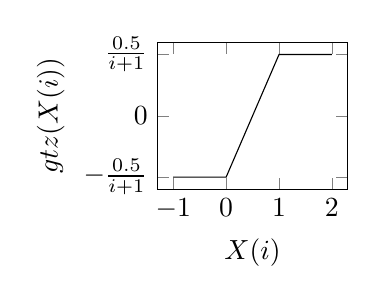
\begin{tikzpicture}[baseline=0.8cm]
    \begin{axis}[width=4cm,xlabel={$X(i)$},xtick={-1,0,1,2},ylabel={$\clipfn(X(i))$},ytick={-0.5,0,0.5},yticklabels={$-\frac{0.5}{i+1}$,$0$,$\frac{0.5}{i+1}$}]
    \addplot[mark=none,samples at={-1,0,1,2}] { min(0.5, x-0.5)-min(0,x) };
    \end{axis}
    \end{tikzpicture}\]

    Observe that $\clipfn(C_2(i)-C_1(i)+0.5)$ equals $\frac{0.5}{i+1}$ if $C_1(i)\leq C_2(i)$, and $-\frac{0.5}{i+1}$ otherwise.
    This is because the counts $C_1(i),C_2(i)$ must be integers, so if $C_1(i)\leq C_2(i)$, then $C_2(i)-C_1(i)+0.5\geq 0.5$, and the expression will evaluate to $\frac{0.5}{i+1}$. Otherwise, $C_2(i)-C_1(i)+0.5<-0.5$, and the expression will evaluate to $-\frac{0.5}{i+1}$.

    It is straightforward, then, to use the construction for $\min$/$\max$ from above to produce a feed-forward layer that computes $\clipfn\left(C_2(i)-C_1(i)\right)$. Essentially, we use $W_1$ to compute the values (using the pre-existing values from the residual stream)

    \[\frac{0.5}{i+1}, \frac{C_2(i)-C_1(i)+0.5}{i+1}, -\frac{C_2(i)-C_1(i)+0.5}{i+1}\]

    Then we use $W_2$ to compute

    \[\frac{0.5}{i+1}+\ReLU\left(\frac{0.5}{i+1}-\frac{C_2(i)-C_1(i)+0.5}{i+1}\right)-\ReLU\left(\frac{0.5}{i+1}-\frac{C_2(i)-C_1(i)-0.5}{i+1}\right)\]
    which equals $\clipfn(C_2(i)-C_1(i))$ as desired.

    Similarly, it is straightforward to construct a feed-forward layer to compare linear combinations of count terms. That is, for disjoint sets of indices $K_1$ and $K_2$, to compute
    \[\clipfn\left(\sum_{k\in K_2} c_{k} \cdot C_k(i) -\sum_{k\in K_1} c_{k} \cdot C_k(i)\right).\]

    So we can construct a feed-forward layer $f:\R^d\to\R^d$ that computes in each dimension $i$ the following

    \[f\left(\begin{bmatrix}
        v_1\\
        v_2\\
        \vdots\\
        v_{2k_3-1}\\
        v_{2k_3}\\
        \vdots\\
        v_{d-1}\\
        v_{d}\\
    \end{bmatrix}\right) =\begin{bmatrix}
        \clipfn(v_1)\\
        \clipfn(v_2)\\
        \vdots\\
        \clipfn\left(\sum_{k\in K_2} c_{k} \cdot C_k(i) -\sum_{k\in K_1} c_{k} \cdot C_k(i)\right)\\
        \clipfn\left(\sum_{k\in K_2} c_{k} \cdot C_k(i) -\sum_{k\in K_1} c_{k} \cdot C_k(i)\right)\\
        \vdots\\
        \clipfn(v_{d-1})\\
        \clipfn(v_{d})\\
    \end{bmatrix}. \]

    This truncates all positive values in the residual stream at this point to be $\frac{0.5}{i+1}$ at position~$i$, and all nonpositive values to be $-\frac{0.5}{i+1}$. As a result, the next application of LayerNorm (with appropriate parameter settings) scales every single value to $\pm 1$. In particular, all previously-computed Boolean values are preserved, and the newly-computed dimensions $2k_3-1,2k$ hold the correct Boolean value based on the desired comparison